\chapter{DHCPv4}

\section{Operation}

DHCPv4 works in a client/server mode. When a client communicates with a DHCPv4 server, the server assigns or leases an IPv4 address to that client. The client connects to the network with that leased IP address until the lease expires.\\

The client must contact the DHCP server periodically to extend the lease. This lease mechanism ensures that clients that move or power off do not keep addresses that they no longer need. When a lease expires, the DHCP server returns the address to the pool where it can be reallocated as necessary.\\

\subsection{Lease origination}

When the client wants to join a network, it begins DORA\footnote{DORA = Discovery, Offer, Request, Acknowledgement} process to obtain a lease.

\begin{enumerate}
\item A client starts the process with a broadcast \textbf{DHCP-DISCOVER} message to finds available DHCPv4 servers.

\item When the DHCPv4 server receives a DHCP-DISCOVER message, it reserves an available IPv4 address to lease to the client. It then sends a \textbf{DHCP-OFFER} message to the requesting client. At the same time, the server caches the MAC address and the leased IPv4 address of the requesting client to create an ARP entry.

\item When the client receives the DHCP-OFFER from the server, it broadcasts \textbf{DHCP-REQUEST} messages. This message serves as an acceptance notice to the selected server and an implicit decline to any other servers.

\item On receiving the DHCP-REQUEST message, the server verifies the lease information with an ICMP ping to that address to ensure it is not being used already. If there is \emph{no} ICMP echo reply, then the address is not being used by any client. Otherwise, that address is being used and the server has to send DHCP-OFFER again.

\item DHCP server sends  unicast \textbf{DHCP-ACK} message to the client. This message informs the client that the IP address is valid. Because The DHCP-ACK message is a duplicate of the DHCP-OFFER, it also provides IP information for the client.

\item When the client receives the DHCPACK message, it performs an ARP lookup for the assigned address. If there is \emph{no} reply to the ARP request, the client knows that the IPv4 address is valid and starts using it as its own.
\end{enumerate}

Sometimes, two clients use the same IPv4 address. This create a \textbf{conflict}. In such case, the server uses the ping command to detect the clients that experiencing address conflict. After that, the client uses ARP to detect conflicts. When an address conflict is detected, the address is \emph{removed} from the pool and not assigned until an administrator resolves the conflict. 

\subsection{Lease renewal}

\begin{enumerate}
\item Before the lease expires, the client sends a \textbf{DHCP-REQUEST} message directly to DHCPv4 server. 

\item On receiving the DHCP-REQUEST message, the server verifies the lease information by returning a \textbf{DHCP-ACK}.

\item If a DHCP-ACK is not received within a specified amount of time, the client broadcasts another DHCP-REQUEST message so that one of the other DHCPv4 servers can extend the lease.
\end{enumerate}

\subsection{Relay agent}

Sometimes, network clients are not on the same subnet as DHCP servers. Because routers do not forward broadcasts, the DHCP-REQUEST from clients are not sent to DHCP server.\\

Cisco offers a solution called Cisco IOS helper address. This solution enables a router to forward DHCP-REQUEST broadcasts to the DHCPv4 server. When
a router forwards address assignment/parameter requests, it is acting as a DHCPv4 \emph{relay agent}.

\section{Message}

The DHCPv4 message format is used for all DHCPv4 transactions. DHCPv4 messages use \textbf{UDP} port \textbf{67} for server, and \textbf{UDP} port \textbf{68}. In other words, DHCPv4 messages sent from the client to server use UDP source port 68 and destination port 67, DHCPv4 messages sent from server to client use UDP source port 67 and destination port 68. \\

The figure shows the format of a DHCPv4 message. The fields are as follows:

\begin{itemize}
\item \textbf{OP code} specifies general type of message: request (1), reply (2).

\item \textbf{Hardware type:} Ethernet (1), Frame Relay (15), Serial (20)

\item \textbf{Hop} controls the forwarding of messages. Set to 0 by a client before transmitting a request.

\item \textbf{Transaction identifier} used by client to match the request with replies from DHCPv4 server.

\item \textbf{Seconds:} amount of time (in seconds) elapsed since a client attempted to acquire or renew a lease.

\item \textbf{Flag} is used by a client that does not know its IPv4 address when it sends a request. Only one of the 16 bits—the broadcast flag—is used. A value of 1 in this field tells the DHCPv4 server or relay agent receiving the request that the reply should be sent as a broadcast.

\end{itemize}

\begin{figure}[hbtp]
\caption{DHCPv4 message format}
\centering
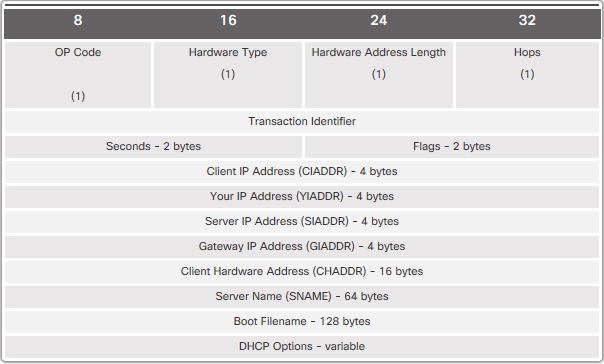
\includegraphics[ width=0.8\textwidth ]{pictures/DHCPmessage.PNG}
\end{figure}

\paragraph{DHCP-DISCOVER:}When the client boots, it has no way of knowing the subnet to which it belongs. Therefore, destination
IPv4 address of DCHP-DISCOVER is 255.255.255.255, the destination MAC address is FF:FF:FF:FF:FF:FF. The source MAC address is the MAC address of the client. The client does not have a configured IPv4 address yet, so the source IPv4 address is 0.0.0.0 

\paragraph{DHCP-OFFER} contains initial configuration information for the client: IPv4 address for client, subnet mask, lease duration, and IPv4 address of the DHCPv4 server. The DHCPOFFER message can be configured to include other information, such as the lease renewal time and DNS address.


\section{Configuration}

\subsection{DHCPv4 server}

\begin{description}
\item[Step 1.] \textbf{Exclude addresses:} Some IPv4 addresses in a pool are assigned to network devices that require static address assignments. Therefore, these IPv4 addresses should not be assigned to other devices.

\begin{verbatim}
R1(config)# ip dhcp excluded-address <ip-address>
R1(config)# ip dhcp excluded-address 192.168.10.1

R1(config)# ip dhcp excluded-address <range-of-address>
R1(config)# ip dhcp excluded-address 192.168.10.1 192.168.10.9
\end{verbatim}

\item[Step 2.] \textbf{Configure address pool:} Define a pool of addresses to assign to clients.

\begin{verbatim}
R1(config)# ip dhcp pool <pool-name>
R1(dhcp-config)# network <network-range>

R1(config)# ip dhcp pool LAN-POOL-1
R1(dhcp-config)# network 192.168.10.0 255.255.255.0
\end{verbatim}

\item[Step 3.] Define the default gateway router for clients. 

\begin{verbatim}
R1(dhcp-config)# default-router 192.168.10.1
\end{verbatim}

\item[Step 4.] \textbf{Relay agent:} If network clients are not on the same subnet as DHCP servers, configure the default gateway as a relay agent.

\begin{verbatim}
R1(config)# interface g0/0
R1(config-if)# ip helper-address 192.168.11.6
\end{verbatim}

\item[Step 4 (Optional)] Other DHCP specifics

\begin{verbatim}
R1(dhcp-config)# dns-server 192.168.11.5
R1(dhcp-config)# domain-name example.com
\end{verbatim}

\item[Step 5.] Verification: The \verb|show ip dhcp binding| command displays a list of all IPv4 address to MAC address bindings that have been provided by the DHCPv4 service. The \verb|show ip dhcp server statistics| command verifies that messages are being received or sent by the router. The \verb|show ip dhcp conflict| command displays all address conflicts recorded by the DHCPv4 server.

\begin{verbatim}
R1# show run | sec dhcp
R1# show ip dhcp binding
R1# show ip dhcp statistics
R1# show ip dhcp conflict
\end{verbatim}

\end{description}

\note  If there is a switch between the client and the DHCPv4 server, and the client is unable to obtain the DHCP configuration, switch port configuration issues may be the cause. These causes may include issues from trunking and channeling, STP, and RSTP. \emph{PortFast} and \emph{Edge port} configurations resolve the most common DHCPv4 client issues that occur with an initial installation of a Cisco switch.

\subsection{DHCPv4 client}

Routers in small office/home office (SOHO) and branch sites have to be configured (by ISP) as DHCPv4 clients in a similar manner to client computers. In the simplest configuration, the Ethernet interface (not Serial interface) of the router is used to connect to a cable or DSL modem. To configure an Ethernet interface of a router as a DHCP client, use the following command:

\begin{verbatim}
SOHO(config)# interface g0/1
SOHO(config-if)# ip address dhcp
SOHO(config-if)# no shutdown
\end{verbatim}


\chapter{DHCPv6}

\section{General Operation}

When the client boots up, it sends DHCPv6 SOLICIT message to \textbf{FF02::1:2}, which is the multicast all-DHCPv6-server address. One or more servers respond with a DHCPv6 ADVERTISE unicast message to inform the client that the server is available for DHCPv6 service. The client responds with either a DHCPv6 REQUEST or a DHCPv6 INFORMATION-REQUEST unicast message: 

\begin{itemize}
\item DHCPv6 INFORMATION-REQUEST unicast message is used for Stateless DHCPv6 (i.e. SLAAC, Stateless DHCPv6 and SLAAC) to request only additional information, such as DNS server addresses, domain name.
\item DHCPv6 REQUEST unicast message is used for Stateful DHCPv6 to ask for all IP configuration parameters from the server.
\end{itemize}

The server sends a DHCPv6 REPLY unicast message to the client containing the information requested in the DHCPv6 REQUEST or DHCPv6 INFORMATION REQUEST message.

\section{SLAAC}

Stateless Address AutoConfiguration (SLAAC) is enabled by default. Both the M flag and the O flag are set to 0 in the RA. In SLAAC, a host automatically obtains its IP configuration from an IPv6-enabled router. The host generates its own global unicast IPv6 address. A DHCPv6 server is not required. SLAAC operation includes the following steps:

\begin{enumerate}
\item Client asks for IPv6 configuration by sending an RS to the router R1.
\item R1 receives the RS message and responds with an RA message.
\item PC1 receives the RA, and uses the information in the message to create its own IPv6 global unicast address. 
\item Because SLAAC is a stateless process, PC1 must verify that this newly created IPv6 address is unique using DAD process.
\end{enumerate}

\begin{figure}[hbtp]
\caption{Verify SLAAC method}
\centering
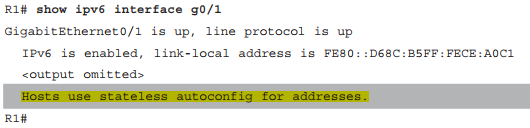
\includegraphics[scale=0.8]{pictures/SLAAC.PNG}
\end{figure}


To configure SLAAC, use the following commands:

\begin{verbatim}
R1(config)# ipv6 unicast-routing
R1(config)#
R1(config)# interface g0/1
R1(config-if)# ipv6 nd managed-config-flag
R1(config-if)# ipv6 nd other-config-flag
R1(config-if)# end
R1# show ipv6 dhcp pool 
R1# show ipv6 interface
R1# debug ipv6 dhcp detail
\end{verbatim}

\section{SLAAC and Stateless DHCPv6}

A host obtains IP configuration (prefix, prefix-length, default gateway) using SLAAC and additional information (DNS server, domain name, etc.) from a stateless DHCPv6 server. The host generates its own global unicast IPv6 address. \\

There are four steps to configure a router as a DHCPv6 server:

\begin{enumerate}
\item Enable IPv6 Routing using \verb|ipv6 unicast-routing| command
\item Use \verb|ipv6 dhcp pool <pool-name>| command to create a pool and enter the router in DHCPv6 configuration mode
\item (Optional) In DHCPv6 configuration mode, configure DNS server address (\verb|dns-server <ip-address>|) and domain name (\verb|domain-name <name>|).
\item In the interface configuration mode, we bind the DHCPv6 pool to the interface using \verb|ipv6 dhcp server <pool-name>|
\item For stateless DHCPv6, the O flag is 1 and the M flag is 0, therefore, to indicate stateless DHCPv6, use the \verb|ipv6 nd other-config-flag| in router interface configuration mode.
\end{enumerate}

\begin{figure}[hbtp]
\caption{Verify Stateless DHCPv6 method}
\centering
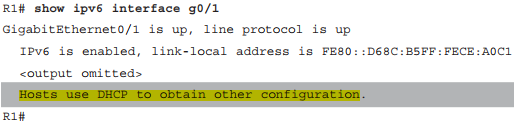
\includegraphics[scale=0.8]{pictures/Stateless-DHCPv6.PNG}
\end{figure}


\begin{verbatim}
R1(config)# ipv6 unicast-routing
R1(config)#
R1(config)# ipv6 dhcp pool IPV6-STATELESS
R1(config-dhcpv6)# dns-server 2001:db8:cafe:aaaa::5
R1(config-dhcpv6)# domain-name example.com
R1(config-dhcpv6)# exit
R1(config)#
R1(config)# interface g0/1
R1(config-if)# ipv6 address 2001:db8:cafe:1::1/64
R1(config-if)# ipv6 dhcp server IPV6-STATELESS
R1(config-if)# ipv6 nd other-config-flag
R1(config-if)# end
R1# show ipv6 dhcp pool 
R1# show ipv6 interface
R1# debug ipv6 dhcp detail
\end{verbatim}

The \verb|show ipv6 dhcp pool| command verifies the name of the DHCPv6 pool and its parameters. The \verb|show ipv6 interface| command  confirms that the interface has ``Stateless address autoconfig enabled'' and has an IPv6 global unicast address. 

\section{Stateful DHCPv6}

In stateful DHCPv6, all IP information information must be obtained from a stateful DHCPv6 server. However, the default router information is not from the DHCPv6 server, but
it was determined by using the source IPv6 address from the RA message. This is known as \emph{stateful} DHCPv6 because the DHCPv6 server maintains IPv6 state information.\\

DHCPv6 messages from the server to the client use \textbf{UDP} destination port \textbf{546}. The client sends DHCPv6 messages to the server using \textbf{UDP} destination port \textbf{547}.\\

There are four steps to configure a router as a DHCPv6 server:

\begin{enumerate}
\item Enable IPv6 Routing using \verb|ipv6 unicast-routing| command
\item Use \verb|ipv6 dhcp pool <pool-name>| command to create a pool and enter the router in DHCPv6 configuration mode
\item In DHCPv6 configuration mode, \verb|address prefix <prefix/length> lifetime <time> <preferred-time>|. The \verb|lifetime| option indicates the valid and preferred lease times in seconds.
\item (Optional) Configure DNS server address (\verb|dns-server <ip-address>|) and domain name (\verb|domain-name <name>|).
\item In the interface configuration mode, we bind the DHCPv6 pool to the interface using \verb|ipv6 dhcp server <pool-name>|
\item Because the M flag indicates whether or not to use stateful DHCPv6 and the O flag is not involved, to signify stateful DHCPv6, we set the M flag as 1 using \verb|ipv6 nd managed-config-flag| in router interface configuration mode.
\end{enumerate}

\begin{figure}[hbtp]
\caption{Verify stateful DHCPv6}
\centering
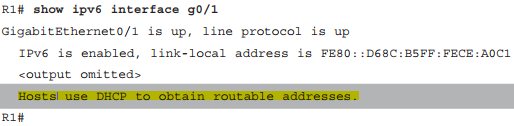
\includegraphics[scale=0.8]{pictures/Stateful-DHCPv6.PNG}
\end{figure}


\begin{verbatim}
R1(config)# ipv6 unicast-routing
R1(config)#
R1(config)# ipv6 dhcp pool IPV6-STATEFUL
R1(config-dhcpv6)# address prefix 2001:DB8:CAFE:1::/64 lifetime infinite infinite
R1(config-dhcpv6)# dns-server 2001:db8:cafe:aaaa::5
R1(config-dhcpv6)# domain-name example.com
R1(config-dhcpv6)# exit
R1(config)#
R1(config)# interface g0/1
R1(config-if)# ipv6 address 2001:db8:cafe:1::1/64
R1(config-if)# ipv6 dhcp server IPV6-STATEFUL
R1(config-if)# ipv6 nd managed-config-flag
R1(config-if)# end
\end{verbatim}

The \verb|show ipv6 dhcp pool| command verifies the name of the DHCPv6 pool and its parameters. The \verb|show ipv6 dhcp binding| command displays the automatic binding between the link-local address of the client and the address that the server assigns. 

\section{Router as DHCPv6 client}

In the following commands, a Cisco router is used as the stateless DHCPv6 client. The \verb|ipv6 enable| command is used because the router does not yet have a global unicast address. The \verb|ipv6 address autoconfig| command enables automatic configuration of IPv6 addressing using SLAAC. By assumption, the server router is configured for stateless DHCPv6, so it sends an RA message to inform the client router to use stateless DHCPv6 to obtain DNS information.

\begin{verbatim}
R3(config)# interface g0/1
R3(config-if)# ipv6 enable
R3(config-if)# ipv6 address autoconfig
R3(config-if)# end
\end{verbatim}

\section{Relay agent}

If the DHCPv6 server is located on a different network than the client, the IPv6 router can be configured as a DHCPv6 relay agent using \verb|ipv6 dhcp relay destination 2001:db8:cafe:1::6| command in interface configuration mode.

\section{Message}

\paragraph{Router solicitation (RS)} The client sends an RS message to the router. The destination address of the message is \textbf{all-routers} multicast address \textbf{FF02::2}.

\paragraph{Router advertisement (RA)} is sent by routers to provide IP configuration to clients. The RA message includes IPv6 configuration for clients (prefix, prefix-length, DNS server, MTU, and default gateway information). A router sends an RA message periodically (every 200s) or in response to an RS message. RA messages are always sent to the IPv6 \textbf{all-nodes} multicast address \textbf{FF02::1}.\\

The two flags are the Managed Address Configuration flag (M flag) and the Other Configuration flag (O flag). Using different combinations of the M and O flags, RA messages have one of three addressing options for the IPv6 device:

\begin{itemize}
\item SLAAC (M = 0, O = 0)
\item SLAAC and Stateless DHCPv6 (M = 0, O = 1)
\item Stateful DHCPv6 (M = 1)
\end{itemize}


